\documentclass{article}
\usepackage{listings}
\documentclass[a4paper,10pt]{article}
\usepackage{siunitx}
\usepackage{spreadtab}
\usepackage{amsmath}
\usepackage[euler]{textgreek}
\usepackage{url}
\usepackage[siunitx]{circuitikz}
\usepackage{circuitikz}
\usepackage{siunitx}
\usepackage{placeins}
\usepackage{amssymb}
\usepackage{amsmath}

\input{./discussion/fwr_discussion_preamble.tex}
\begin{document}
	\begin{titlepage}
		\centering
		\Huge{Experiment 5} \\
		\huge{Transient Responses of Diodes and Rectifiers} \\
		\vspace{1cm}
		\large{EECS 170A - Lab Bench \#1} \\
		\large{\today} \\
		\vspace{1cm}
		\normalsize{Roman Parise (59611417)} \\
		\normalsize{Krishan Solanki (38154673)} \\
		\normalsize{Jason Wang (42873192)} \\
	\end{titlepage}
\section{Procedure}
\underline{Procedure}

For the second Electronics Lab, the objective is to solder RC circuits on a printed circuit board and then test the circuit as a Lowpass and Highpass Filter. To solder the resistor and capacitor, a soldering iron is used by melting metal onto the ends of the resistor and capacitor on a printed circuit board. After soldering, the output voltage in sine wave mode is measured at different frequencies using the oscilloscope. The Lowpass Filter has a function generator with internal resistance of (50\textOmega) which is in series with a 10k\textOmega resistor. The capacitor in this circuit is in parallel with the oscilloscope. The Highpass filter has a function generator with internal resistance of 50\textOmega  in series with a capacitor. The 10k\textOmega resistor is connected to the negative terminal of the function generator and is also in parallel with the oscilloscope. After taking the measurements, the transfer function ($H_{(s)} = \frac{V_o}{V_{in}$) for both filters are plotted as a function of frequency on a log-log scale. Lastly, the impulse response is measured by sending a pulse signal that is shorter than the RC time constant. The measured responses are then compared to the theoretical responses. \\
\\
\underline{LowPass Filter}
\\
\centerline{ $ H_{(s)} = \frac{V_o}{V_{in}} = \frac{Z_c}{Z_r + Z_c} $ }
\centerline{ $ Z_r = R, Z_c = \frac{1}{sc} $}
\centerline{ $ H_{(s)} = \frac{V_o}{V_{in}} = \frac{\frac{1}{sc}}{R + \frac{1}{sc}} $ }
\begin{equation}
\label{eq:LowPassFunction}
\centerline{ $ H_{(s)} = \frac{V_o}{V_{in}} = \frac{1}{sRC + 1} $ }
\end{equation}
\\
\underline{HighPass Filter}
\\
\centerline{ $ H_{(s)} = \frac{V_o}{V_{in}} = \frac{Z_r}{Z_r + Z_c} $ }
\centerline{ $ Z_r = R, Z_c = \frac{1}{sc} $}
\centerline{ $ H_{(s)} = \frac{V_o}{V_{in}} = \frac{R}{R + \frac{1}{sc}} $ }
\begin{equation}
\label{eq:HighPassFunction}
\centerline{ $ H_{(s)} = \frac{V_o}{V_{in}} = \frac{sRC}{sRC + 1} $ }
\end{equation}





\section{Results and Analysis}
\subsection{Transient Response of Diodes}
% JASON: PLEASE SEPARATE SCHOTTKY, PN-JUNCTION, ETC. INTO DIFFERENT SECTIONS IF YOU CAN. OTHERWISE, DON'T WORRY ABOUT IT.
\subsection{Full-Wave Bridge Rectifier}
\FloatBarrier

\begin{figure}[h!]
\centering
\caption{Full-Wave Bridge Rectifier Circuit}
\label{fig:fwr}
\begin{circuitikz}
	\draw
	( 0 , 4 ) to [ sV , v<=$20Vpp$ ] ( 0 , 0 )
	( 0 , 4 ) -- ( 4 , 4 ) to [ empty diode ] ( 6 , 2 )
	( 2 , 2 ) to [ empty diode ] ( 4 , 4 )
	( 2 , 2 ) to [ empty diode ] ( 4 , 0 )
	( 4 , 0 ) to [ empty diode ] ( 6 , 2 )
	( 4 , 0 ) -- ( 0 , 0 )
	( 2 , 2 ) to [ R = 300 <\ohm> ] ( 6 , 2 )
	( 2 , 2 ) node[label={ [font=\normalsize] above : $-$ } ] { }
	( 6 , 2 ) node[label={ [font=\normalsize] above : $+$ } ] { }
	;
\end{circuitikz}
\end{figure}

\FloatBarrier

Figure (\ref{fig:fwr}) displays a full-wave bridge rectifier circuit. The circuit's specification requires that it take an input sinusoidal signal and produce an output voltage that is the absolute value of that signal with the least amount of error possible. The output voltage is measured over the resistor, which shall be referred to as $R$. In reality, this ideal is not reached. The experiment demonstrates the degree to which the specification is satisfied.
The full-wave bridge rectifier circuit takes advantage of the fact that diodes essentially act as broken circuits when the applied voltage is less than its threshold voltage and act as short circuits when the applied voltage exceeds its threshold voltage. This is a simplification of the Shockley diode model:

\begin{equation}
	\label{eq:shockley_diode}
	I_{diode}( V_{applied} ) = I_0 ( e^{ \frac{qV_{applied}}{k_B T} } - 1 )
\end{equation}

In equation (\ref{eq:shockley_diode}), $I_0$ is the reverse saturation current, $q$ is the elementary charge, $k_B$ is Boltzmann's constant, and $T$ is temperature. A more ideal model treats the diode as the perfect switch described above, namely that the diode acts as a broken circuit unless $V_{applied}$ exceeds its threshold voltage, assumed to be about 0.7\si{\volt} and referred to as $V_{Th}$. Figure (\ref{fig:ideal_vs_shock}) below compares these two models in a graph. The graph demonstrates that this more idealized model accurately characterizes the behavior of the diode. It shall be used instead to describe the diode's characteristics.

\FloatBarrier

\begin{figure}[h!]
	\centering
	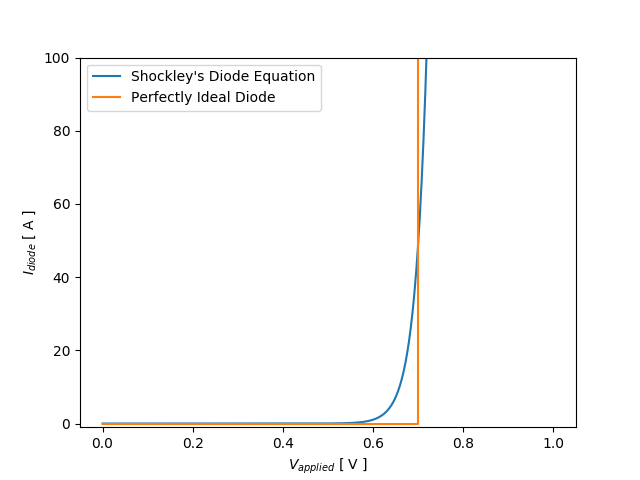
\includegraphics[scale=0.75]{../images/ideal_diode.PNG}
	\caption{Shockley Diode Model vs. Perfectly Ideal Diode}
	\label{fig:ideal_vs_shock}
\end{figure}

\FloatBarrier

{\footnotesize $I_0$ is set to 0.1\si{\nano\ampere}. Temperature is assumed to be 300\si{\kelvin}. Threshold voltage of perfectly ideal model is assumed to be 0.7\si{\volt}. }

\FloatBarrier

A diode is said to be enabled when the applied source voltage, which shall be called $V_{A}$, meets or exceeds its threshold voltage. Enabled diodes are drawn in green. Two cases are to be considered: when $V_{A} > 2V_{Th}$ and when $V_{A} < 2V_{Th}$. $2V_{Th}$ must be used since the voltage must enabled two diodes in series as seen in the figures below. Note that $|V_{A}| < 2V_{Th}$ is trivial since no voltage drops over the load resistor $R$.

When $V_{A} > 2V_{Th}$, the diodes in figure (\ref{fig:v_app_high}) are enabled. The voltage measured over the resistor is clearly positive due to the direction of positive current flow. The positive current flow direction is indicated by an arrow.

\FloatBarrier

\begin{figure}[h!]
\centering
\caption{Full-Wave Rectifier when $V_{A} > 2V_{Th}$}
\label{fig:v_app_high}
\begin{circuitikz}
	\draw
	( 0 , 4 ) to [ sV , v<=$20Vpp$ ] ( 0 , 0 )
	( 0 , 4 ) -- ( 4 , 4 ) to [ empty diode , color = green ] ( 6 , 2 )
	( 2 , 2 ) to [ empty diode ] ( 4 , 4 )
	( 2 , 2 ) to [ empty diode , color = green ] ( 4 , 0 )
	( 4 , 0 ) to [ empty diode ] ( 6 , 2 )
	( 4 , 0 ) -- ( 0 , 0 )
	( 2 , 2 ) to [ R = 300 <\ohm> , i<_=$I$ ] ( 6 , 2 )
	( 2 , 2 ) node[label={ [font=\normalsize] above : $-$ } ] { }
	( 6 , 2 ) node[label={ [font=\normalsize] above : $+$ } ] { }
	;
\end{circuitikz}
\end{figure}

\FloatBarrier

Figure (\ref{fig:v_app_low}) demonstrates the case when $V_{A} < 2V_{Th}$. Again, the output voltage taken over the resistor is positive due to the direction of positive current flow.

\FloatBarrier

\begin{figure}[h!]
\centering
\caption{Full-Wave Rectifier when $V_{A} < 2V_{Th}$}
\label{fig:v_app_low}
\begin{circuitikz}
	\draw
	( 0 , 4 ) to [ sV , v<=$20Vpp$ ] ( 0 , 0 )
	( 0 , 4 ) -- ( 4 , 4 ) to [ empty diode ] ( 6 , 2 )
	( 2 , 2 ) to [ empty diode , color = green ] ( 4 , 4 )
	( 2 , 2 ) to [ empty diode ] ( 4 , 0 )
	( 4 , 0 ) to [ empty diode , color = green ] ( 6 , 2 )
	( 4 , 0 ) -- ( 0 , 0 )
	( 2 , 2 ) to [ R = 300 <\ohm> , i<_=$I$ ] ( 6 , 2 )
	( 2 , 2 ) node[label={ [font=\normalsize] above : $-$ } ] { }
	( 6 , 2 ) node[label={ [font=\normalsize] above : $+$ } ] { }
	;
\end{circuitikz}
\end{figure}

\FloatBarrier

A more quantitative description of this behavior can be obtained. In the $V_{A} > 2V_{Th}$ case, Kirchhoff's voltage law may be applied:

\FloatBarrier

\begin{figure}[h!]
\centering
\caption{Kirchhoff's Voltage Law for $V_{A} > 2V_{Th}$}
\label{fig:kvl_app_high}
\begin{circuitikz}
	\draw
	( 0 , 4 ) to [ sV , v<=$20Vpp$ ] ( 0 , 0 )
	( 0 , 4 ) -- ( 4 , 4 ) to [ empty diode , color = green ] ( 6 , 2 )
	( 2 , 2 ) to [ empty diode , color = green ] ( 4 , 0 )
	( 4 , 0 ) -- ( 0 , 0 )
	( 2 , 2 ) to [ R = 300 <\ohm> , i<_=$I$ ] ( 6 , 2 )
	( 2 , 2 ) node[label={ [font=\normalsize] above : $-$ } ] { }
	( 6 , 2 ) node[label={ [font=\normalsize] above : $+$ } ] { }
	( 1.5 , 1 ) node[scale=3]{$\circlearrowright$}
	;
\end{circuitikz}
\end{figure}

\FloatBarrier

\begin{equation}
	\label{eq:kvl_va_gt_2vth}
	+V_{A} - V_{Th} - V_{out} - V_{Th} = 0 \rightarrow V_{out} = V_{A} - 2V_{Th}
\end{equation}

The same method can be applied to the $V_{A} < 2V_{Th}$ case.

\FloatBarrier

\begin{figure}[h!]
\centering
\caption{Kirchhoff's Voltage Law for $V_{A} > 2V_{Th}$}
\label{fig:kvl_app_low}
\begin{circuitikz}
	\draw
	( 0 , 4 ) to [ sV , v<=$20Vpp$ ] ( 0 , 0 )
	( 0 , 4 ) -- ( 4 , 4 )
	( 2 , 2 ) to [ empty diode , color = green ] ( 4 , 4 )
	( 4 , 0 ) to [ empty diode , color = green ] ( 6 , 2 )
	( 4 , 0 ) -- ( 0 , 0 )
	( 2 , 2 ) to [ R = 300 <\ohm> , i<_=$I$ ] ( 6 , 2 )
	( 2 , 2 ) node[label={ [font=\normalsize] above : $-$ } ] { }
	( 6 , 2 ) node[label={ [font=\normalsize] above : $+$ } ] { }
	( 1.5 , 1 ) node[scale=3]{$\circlearrowright$}
	;
\end{circuitikz}
\end{figure}

\FloatBarrier

\begin{equation}
	\label{eq:kvl_va_lt_2vth}
	+V_{A} + V_{Th} + V_{out} + V_{Th} = 0 \rightarrow V_{out} = - V_{A} - 2V_{Th}
\end{equation}

These behaviors can be generalized in the following result for the output voltage of the full-wave rectifier circuit in figure (\ref{fig:fwr}):

\begin{equation}
	\label{eq:fwr_eq}
	V_{out}(V_{A}) =
	\begin{cases}
		|V_{A}| - 2V_{Th} , & |V_{A}| > 2V_{Th} \\
		0 , & \text{otherwise}
	\end{cases}
\end{equation}

A plot of the expected output voltage against the input voltage is shown in figure (\ref{fig:expected_out_vs_in_fwr}):

\FloatBarrier

\begin{figure}[h!]
	\centering
	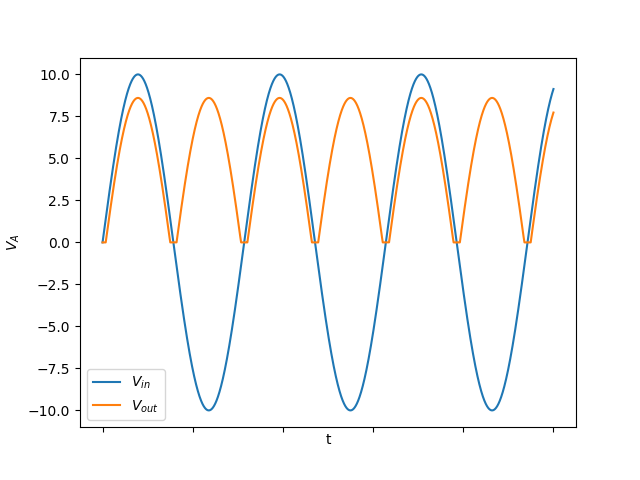
\includegraphics[scale=0.75]{../images/full_wave_rect.PNG}
	\caption{Full-Wave Bridge Rectifier Expected Result}
	\label{fig:expected_out_vs_in_fwr}
\end{figure}

\FloatBarrier


\section{Discussion}
\subsection{Transient Response of Diodes}
\subsection{Full-Wave Bridge Rectifier}
The full-wave bridge rectifier results align quite well with theory. However, the peak measurement does have slightly more error than the trough measurement. These errors are a result of either an asymmetry in the source voltage or an asymmetry in the threshold voltages of the diodes. The former is not possible to prove due to the fact that the source voltage is not probed in the experiment. However, if the sinusoidal source voltage's peak is higher than the reported value on the power supply, this would explain why the measured voltage for the output voltage's peak is higher than expected. Furthermore, the diodes may differ in threshold voltage. Differences in threshold voltage are a result of either temperature, material, or doping variations:

\begin{align*}
	\label{eq:vbi}
	V_{bi} = \frac{k_BT}{q} ln( \frac{N_AN_D}{(n_{i}(T))^2} )
\end{align*}

Temperature is likely not the cause since the temperature in the room in which the experiment is conducted is essentially uniform, which would not explain the asymmetry in the measurements. A better explanation is that the doping concentrations vary slightly from diode to diode due to slight nonidealities in the manufacturing process. So, the diodes along the enabled path when the source voltage is positive could have slightly lower threshold voltages than the diodes along the other path.

\section{Appendix}
The following script is used to generate the theoretical full-wave recitifer plot in figure (\ref{fig:expected_out_vs_in_fwr}):
\lstinputlisting[breaklines]{./scripts/full_wave_rect.py}
The following script is used to generate tables (\ref{tab:peak_n_trough}) and (\ref{tab:theory_vs_practice}):
\lstinputlisting[breaklines]{./scripts/fwr_data.py}
Lastly, this script is used to generate figure (\ref{fig:ideal_vs_shock}):
\lstinputlisting[breaklines]{./scripts/gen_ideal_diode.py}
\end{document}
